\begin{tikzpicture}[
    node distance = 1cm and 2cm,
    usecase/.style={ellipse, draw, minimum width=4.5cm, minimum height=0.7cm, align=center, font=\small},
    link/.style={draw, thick}
]
% Boundary
\draw[thick] (0, 0) rectangle (9, -13.5);
\node at (4.5, -0.6) {\textbf{Medical Office Management}};

% Medical Officer Actor
\node (medOfficer) at (-2, -5.5) {
    \begin{tikzpicture}[scale=0.5]
        \draw[thick] (0,1.2) circle (0.4cm); \draw[thick] (0,0.8) -- (0,-0.8);
        \draw[thick] (-0.8,0.4) -- (0.8,0.4); \draw[thick] (0,-0.8) -- (-0.5,-1.8); \draw[thick] (0,-0.8) -- (0.5,-1.8);
        \node at (0,-2.5) {\small Medical Officer};
    \end{tikzpicture}
};

% Admin Actor
\node (admin) at (11, -5.5) {
    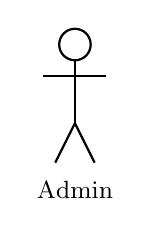
\begin{tikzpicture}[scale=0.5]
        \draw[thick] (0,1.2) circle (0.4cm); \draw[thick] (0,0.8) -- (0,-0.8);
        \draw[thick] (-0.8,0.4) -- (0.8,0.4); \draw[thick] (0,-0.8) -- (-0.5,-1.8); \draw[thick] (0,-0.8) -- (0.5,-1.8);
        \node at (0,-2.5) {\small Admin};
    \end{tikzpicture}
};

% Use Cases
\node[usecase] (uc1) at (4.5, -1.5) {Search Applicant};
\node[usecase] (uc2) at (4.5, -2.6) {Show Applicant's profile};
\node[usecase] (uc3) at (4.5, -3.7) {Admit Applicant};
\node[usecase] (uc4) at (4.5, -4.8) {View Waited Applicants};
\node[usecase] (uc5) at (4.5, -5.9) {View Admitted Applicant};
\node[usecase] (uc6) at (4.5, -7.0) {Update Applicant Info};
\node[usecase] (uc7) at (4.5, -8.1) {Export Applicant list};
\node[usecase] (uc8) at (4.5, -9.2) {Download Official Record};
\node[usecase] (uc9) at (4.5, -10.3) {Insert/ Update Medical Info};
\node[usecase] (uc10) at (4.5, -11.4) {Generate and print Medical \\ report};

% Left Connections
\foreach \i in {uc1,uc2,uc3,uc4,uc5,uc7,uc8,uc9,uc10} \draw[link] (medOfficer.east) -- (\i.west);

% Right Connections
\draw[link] (admin.west) -- (uc6.east);
\draw[link] (admin.west) -- (uc3.east);
\end{tikzpicture}